\section{2.4 GHz Transceiver MAC layer}
\label{group__ro__transceiver__mac}\index{2.4 GHz Transceiver MAC layer@{2.4 GHz Transceiver MAC layer}}
MAC layer code for the MC13192 2.4GHz Transceiver.  
\subsection*{Defines}
\begin{CompactItemize}
\item 
\#define {\bf MC13192\_\-IDLE}~0
\item 
\#define {\bf MC13192\_\-RX}~1
\item 
\#define {\bf MC13192\_\-TX}~2
\item 
\#define {\bf NO\_\-PACKET}~0
\item 
\#define {\bf RX\_\-PACKET}~1
\item 
\#define {\bf TX\_\-PACKET}~2
\item 
\#define {\bf DROP\_\-PACKET}~3
\end{CompactItemize}
\subsection*{Functions}
\begin{CompactItemize}
\item 
void {\bf MC13192\_\-init} ()
\begin{CompactList}\small\item\em Initialize the MC13192 TODO: write detailed code description! \item\end{CompactList}\item 
void {\bf init\_\-rx\_\-pkt\_\-mode} (void)
\begin{CompactList}\small\item\em switch MC13192 to receive mode TODO: write detailed code description! \item\end{CompactList}\item 
int {\bf get\_\-rx\_\-pkt} ({\bf rx\_\-packet\_\-t} $\ast$rx\_\-packet)
\begin{CompactList}\small\item\em read a data paket from MC13192 \item\end{CompactList}\item 
void {\bf MC13192\_\-update\_\-state} (void)
\begin{CompactList}\small\item\em Update the state variable to reflect the state of MC13192. \item\end{CompactList}\item 
int {\bf tx\_\-pkt\_\-mode} ({\bf tx\_\-packet\_\-t} $\ast$tx\_\-packet)
\begin{CompactList}\small\item\em send a data packet TODO: write detailed code description! \item\end{CompactList}\item 
void {\bf cca\_\-modus} (void)
\end{CompactItemize}
\subsection*{Variables}
\begin{CompactItemize}
\item 
uint8\_\-t {\bf mc13192\_\-mode}
\item 
uint8\_\-t {\bf mc13192\_\-state}
\end{CompactItemize}


\subsection{Detailed Description}
MAC layer code for the MC13192 2.4GHz Transceiver. 



\begin{Code}\begin{verbatim} #include <helpers.h> 
\end{verbatim}\end{Code}



This contains functions for intializing the chip and switching its internal states and modes of operation

\begin{Desc}
\item[Author:]Original by Dennis Meiering 2004, ported to AVR by Rainer Ostendorf 2006 \end{Desc}


\subsection{Define Documentation}
\index{ro_transceiver_mac@{ro\_\-transceiver\_\-mac}!DROP_PACKET@{DROP\_\-PACKET}}
\index{DROP_PACKET@{DROP\_\-PACKET}!ro_transceiver_mac@{ro\_\-transceiver\_\-mac}}
\subsubsection{\setlength{\rightskip}{0pt plus 5cm}\#define DROP\_\-PACKET~3}\label{group__ro__transceiver__mac_ge6d21e889b606bda0e96103646e85061}




Definition at line 53 of file transceiver\_\-mac.h.

Referenced by MC13192\_\-update\_\-state().\index{ro_transceiver_mac@{ro\_\-transceiver\_\-mac}!MC13192_IDLE@{MC13192\_\-IDLE}}
\index{MC13192_IDLE@{MC13192\_\-IDLE}!ro_transceiver_mac@{ro\_\-transceiver\_\-mac}}
\subsubsection{\setlength{\rightskip}{0pt plus 5cm}\#define MC13192\_\-IDLE~0}\label{group__ro__transceiver__mac_g1396300cf28dc20aa56390e6782c8530}




Definition at line 46 of file transceiver\_\-mac.h.

Referenced by MC13192\_\-init().\index{ro_transceiver_mac@{ro\_\-transceiver\_\-mac}!MC13192_RX@{MC13192\_\-RX}}
\index{MC13192_RX@{MC13192\_\-RX}!ro_transceiver_mac@{ro\_\-transceiver\_\-mac}}
\subsubsection{\setlength{\rightskip}{0pt plus 5cm}\#define MC13192\_\-RX~1}\label{group__ro__transceiver__mac_g7e0eefa1d6f5111fafc7742caeb9c919}




Definition at line 47 of file transceiver\_\-mac.h.\index{ro_transceiver_mac@{ro\_\-transceiver\_\-mac}!MC13192_TX@{MC13192\_\-TX}}
\index{MC13192_TX@{MC13192\_\-TX}!ro_transceiver_mac@{ro\_\-transceiver\_\-mac}}
\subsubsection{\setlength{\rightskip}{0pt plus 5cm}\#define MC13192\_\-TX~2}\label{group__ro__transceiver__mac_g926b262c765b52f8607f475062d0e79f}




Definition at line 48 of file transceiver\_\-mac.h.\index{ro_transceiver_mac@{ro\_\-transceiver\_\-mac}!NO_PACKET@{NO\_\-PACKET}}
\index{NO_PACKET@{NO\_\-PACKET}!ro_transceiver_mac@{ro\_\-transceiver\_\-mac}}
\subsubsection{\setlength{\rightskip}{0pt plus 5cm}\#define NO\_\-PACKET~0}\label{group__ro__transceiver__mac_g8ac4964a6cca903f40f29b27f71ef9a1}




Definition at line 50 of file transceiver\_\-mac.h.

Referenced by MC13192\_\-init(), and MC13192\_\-update\_\-state().\index{ro_transceiver_mac@{ro\_\-transceiver\_\-mac}!RX_PACKET@{RX\_\-PACKET}}
\index{RX_PACKET@{RX\_\-PACKET}!ro_transceiver_mac@{ro\_\-transceiver\_\-mac}}
\subsubsection{\setlength{\rightskip}{0pt plus 5cm}\#define RX\_\-PACKET~1}\label{group__ro__transceiver__mac_gb2b34141e1e324bb7389e1cd3940a4f1}




Definition at line 51 of file transceiver\_\-mac.h.

Referenced by MC13192\_\-update\_\-state().\index{ro_transceiver_mac@{ro\_\-transceiver\_\-mac}!TX_PACKET@{TX\_\-PACKET}}
\index{TX_PACKET@{TX\_\-PACKET}!ro_transceiver_mac@{ro\_\-transceiver\_\-mac}}
\subsubsection{\setlength{\rightskip}{0pt plus 5cm}\#define TX\_\-PACKET~2}\label{group__ro__transceiver__mac_ga1072634687af8330af48ca3ef23c144}




Definition at line 52 of file transceiver\_\-mac.h.

Referenced by MC13192\_\-update\_\-state().

\subsection{Function Documentation}
\index{ro_transceiver_mac@{ro\_\-transceiver\_\-mac}!cca_modus@{cca\_\-modus}}
\index{cca_modus@{cca\_\-modus}!ro_transceiver_mac@{ro\_\-transceiver\_\-mac}}
\subsubsection{\setlength{\rightskip}{0pt plus 5cm}void cca\_\-modus (void)}\label{group__ro__transceiver__mac_g6d9695bac8eb630174f8254a42f5c526}




Definition at line 84 of file transceiver\_\-mac.c.

References read\_\-from\_\-spi(), uart\_\-puts(), and write\_\-to\_\-spi().

Here is the call graph for this function:\begin{figure}[H]
\begin{center}
\leavevmode
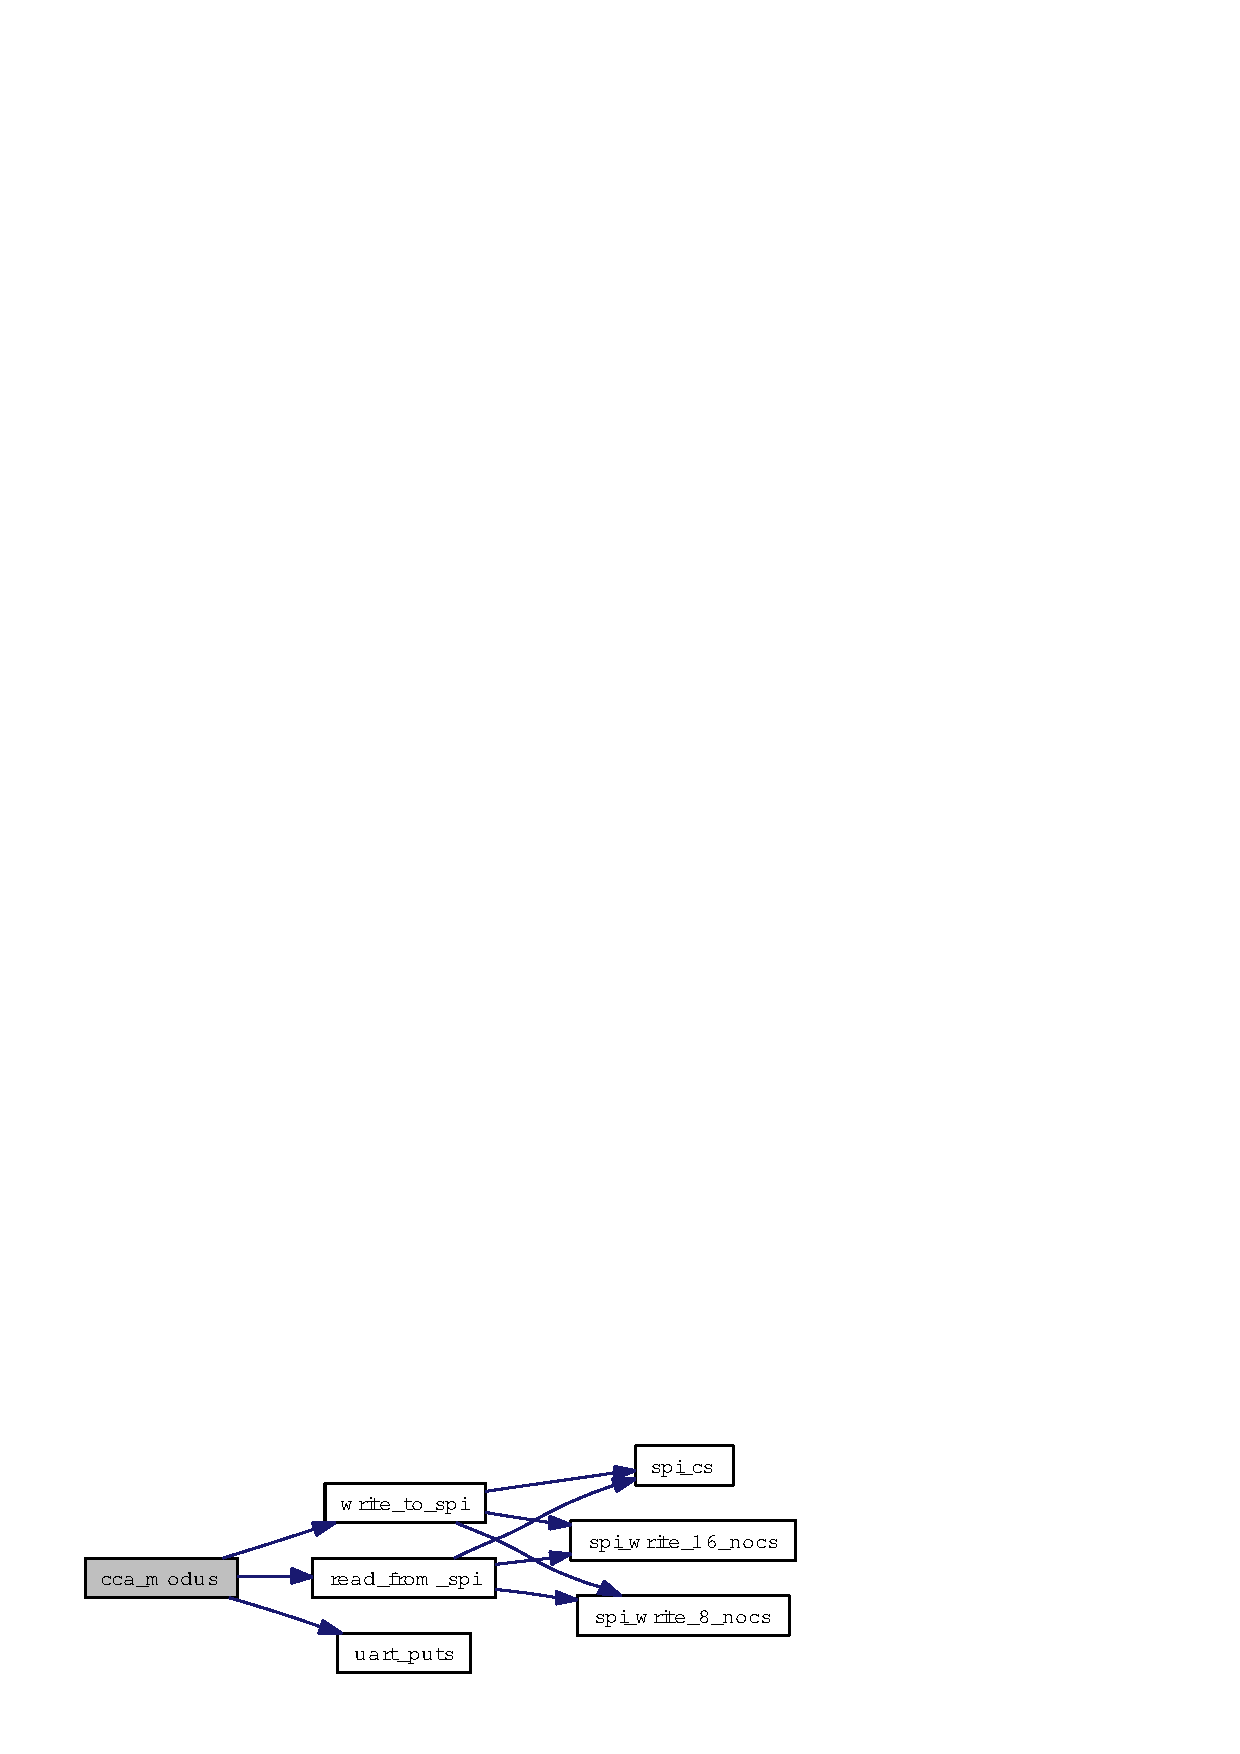
\includegraphics[width=193pt]{group__ro__transceiver__mac_g6d9695bac8eb630174f8254a42f5c526_cgraph}
\end{center}
\end{figure}
\index{ro_transceiver_mac@{ro\_\-transceiver\_\-mac}!get_rx_pkt@{get\_\-rx\_\-pkt}}
\index{get_rx_pkt@{get\_\-rx\_\-pkt}!ro_transceiver_mac@{ro\_\-transceiver\_\-mac}}
\subsubsection{\setlength{\rightskip}{0pt plus 5cm}int get\_\-rx\_\-pkt ({\bf rx\_\-packet\_\-t} $\ast$ {\em rx\_\-packet})}\label{group__ro__transceiver__mac_g067cd80bde03341e70769deee8aa8054}


read a data paket from MC13192 

r

TODO: write detailed code description! \begin{Desc}
\item[Parameters:]
\begin{description}
\item[{\em rx\_\-packet}]Datastructure to save the received data to \end{description}
\end{Desc}
\begin{Desc}
\item[Returns:]1 in every case \end{Desc}


Definition at line 122 of file transceiver\_\-mac.c.

References rx\_\-packet\_\-t::data\-Length, read\_\-from\_\-ram(), and read\_\-from\_\-spi().

Here is the call graph for this function:\begin{figure}[H]
\begin{center}
\leavevmode
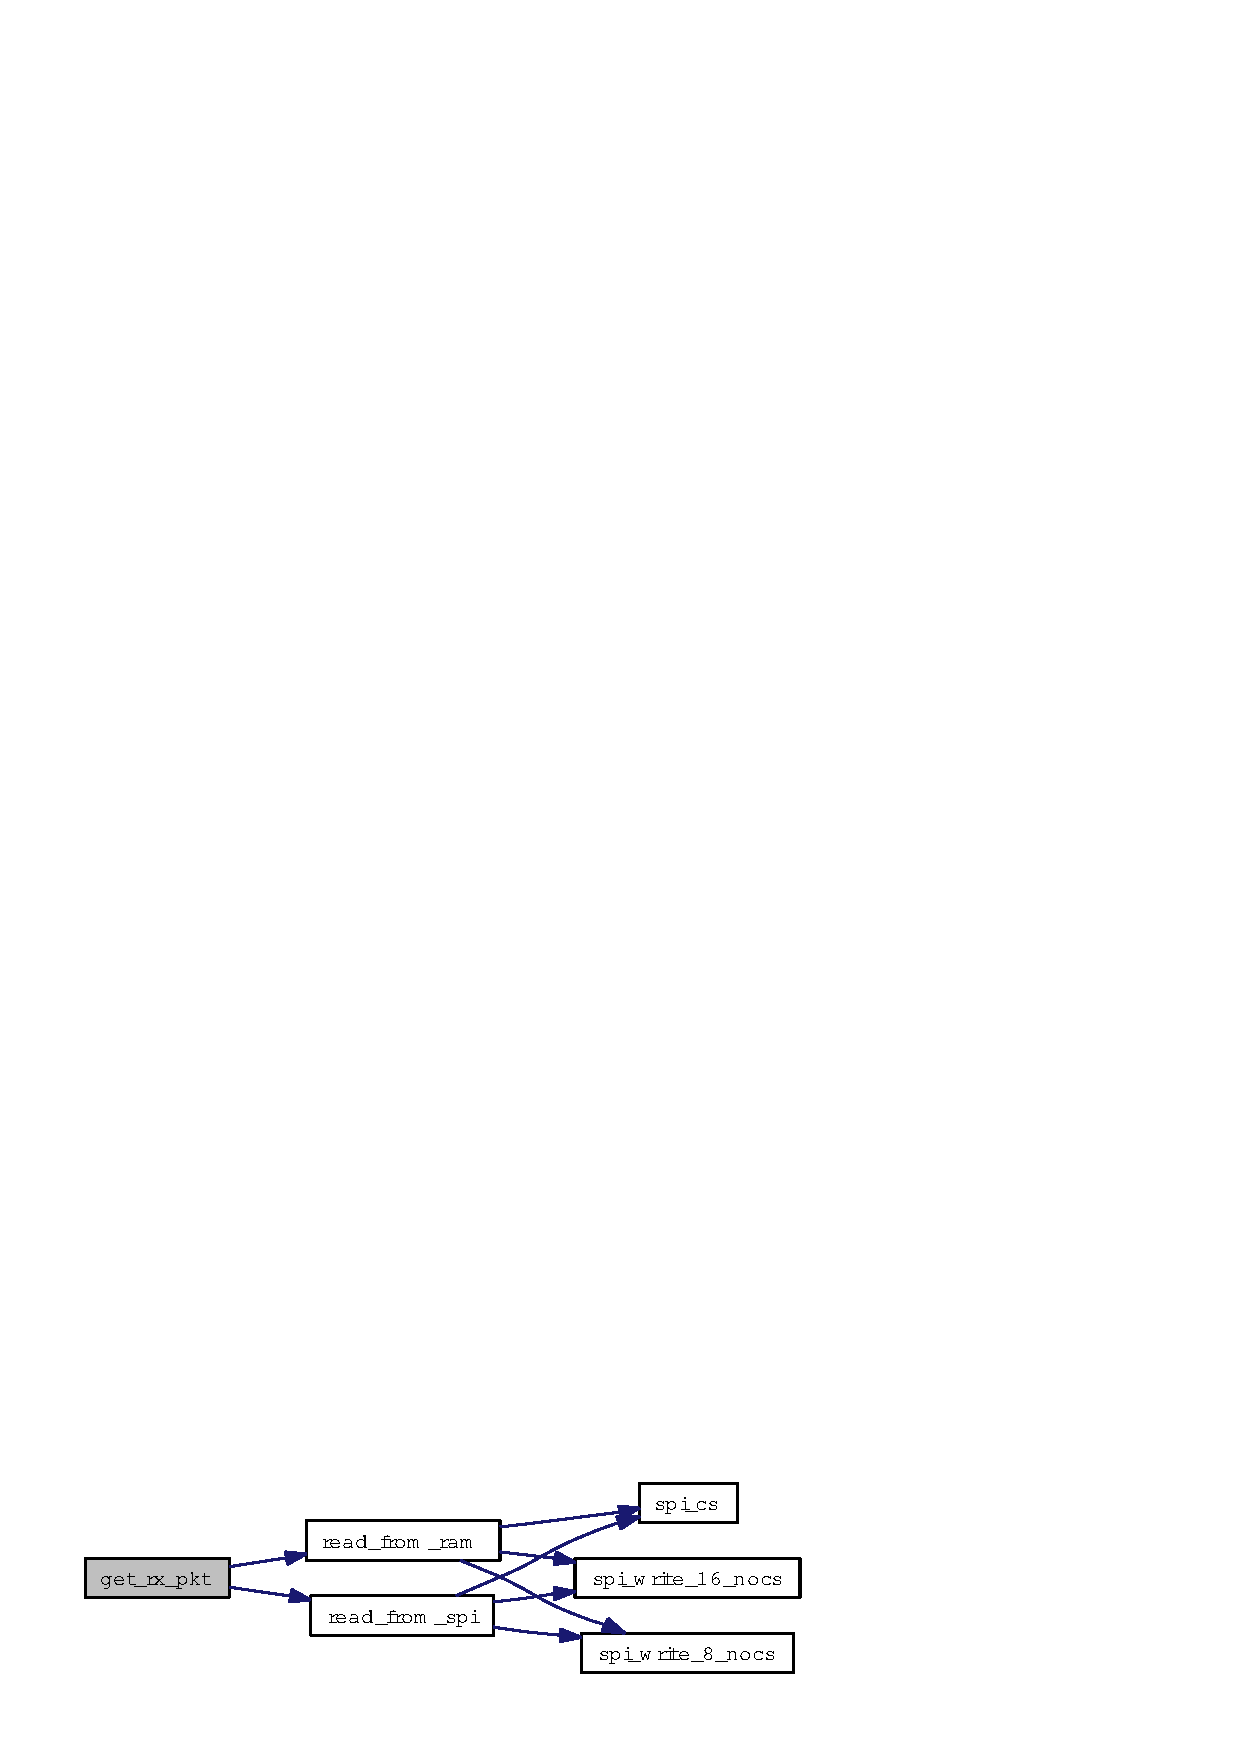
\includegraphics[width=194pt]{group__ro__transceiver__mac_g067cd80bde03341e70769deee8aa8054_cgraph}
\end{center}
\end{figure}
\index{ro_transceiver_mac@{ro\_\-transceiver\_\-mac}!init_rx_pkt_mode@{init\_\-rx\_\-pkt\_\-mode}}
\index{init_rx_pkt_mode@{init\_\-rx\_\-pkt\_\-mode}!ro_transceiver_mac@{ro\_\-transceiver\_\-mac}}
\subsubsection{\setlength{\rightskip}{0pt plus 5cm}void init\_\-rx\_\-pkt\_\-mode (void)}\label{group__ro__transceiver__mac_g0ed60622e56ffb790ac27c0a3aa933ba}


switch MC13192 to receive mode TODO: write detailed code description! 



Definition at line 116 of file transceiver\_\-mac.c.

References write\_\-to\_\-spi().

Here is the call graph for this function:\begin{figure}[H]
\begin{center}
\leavevmode
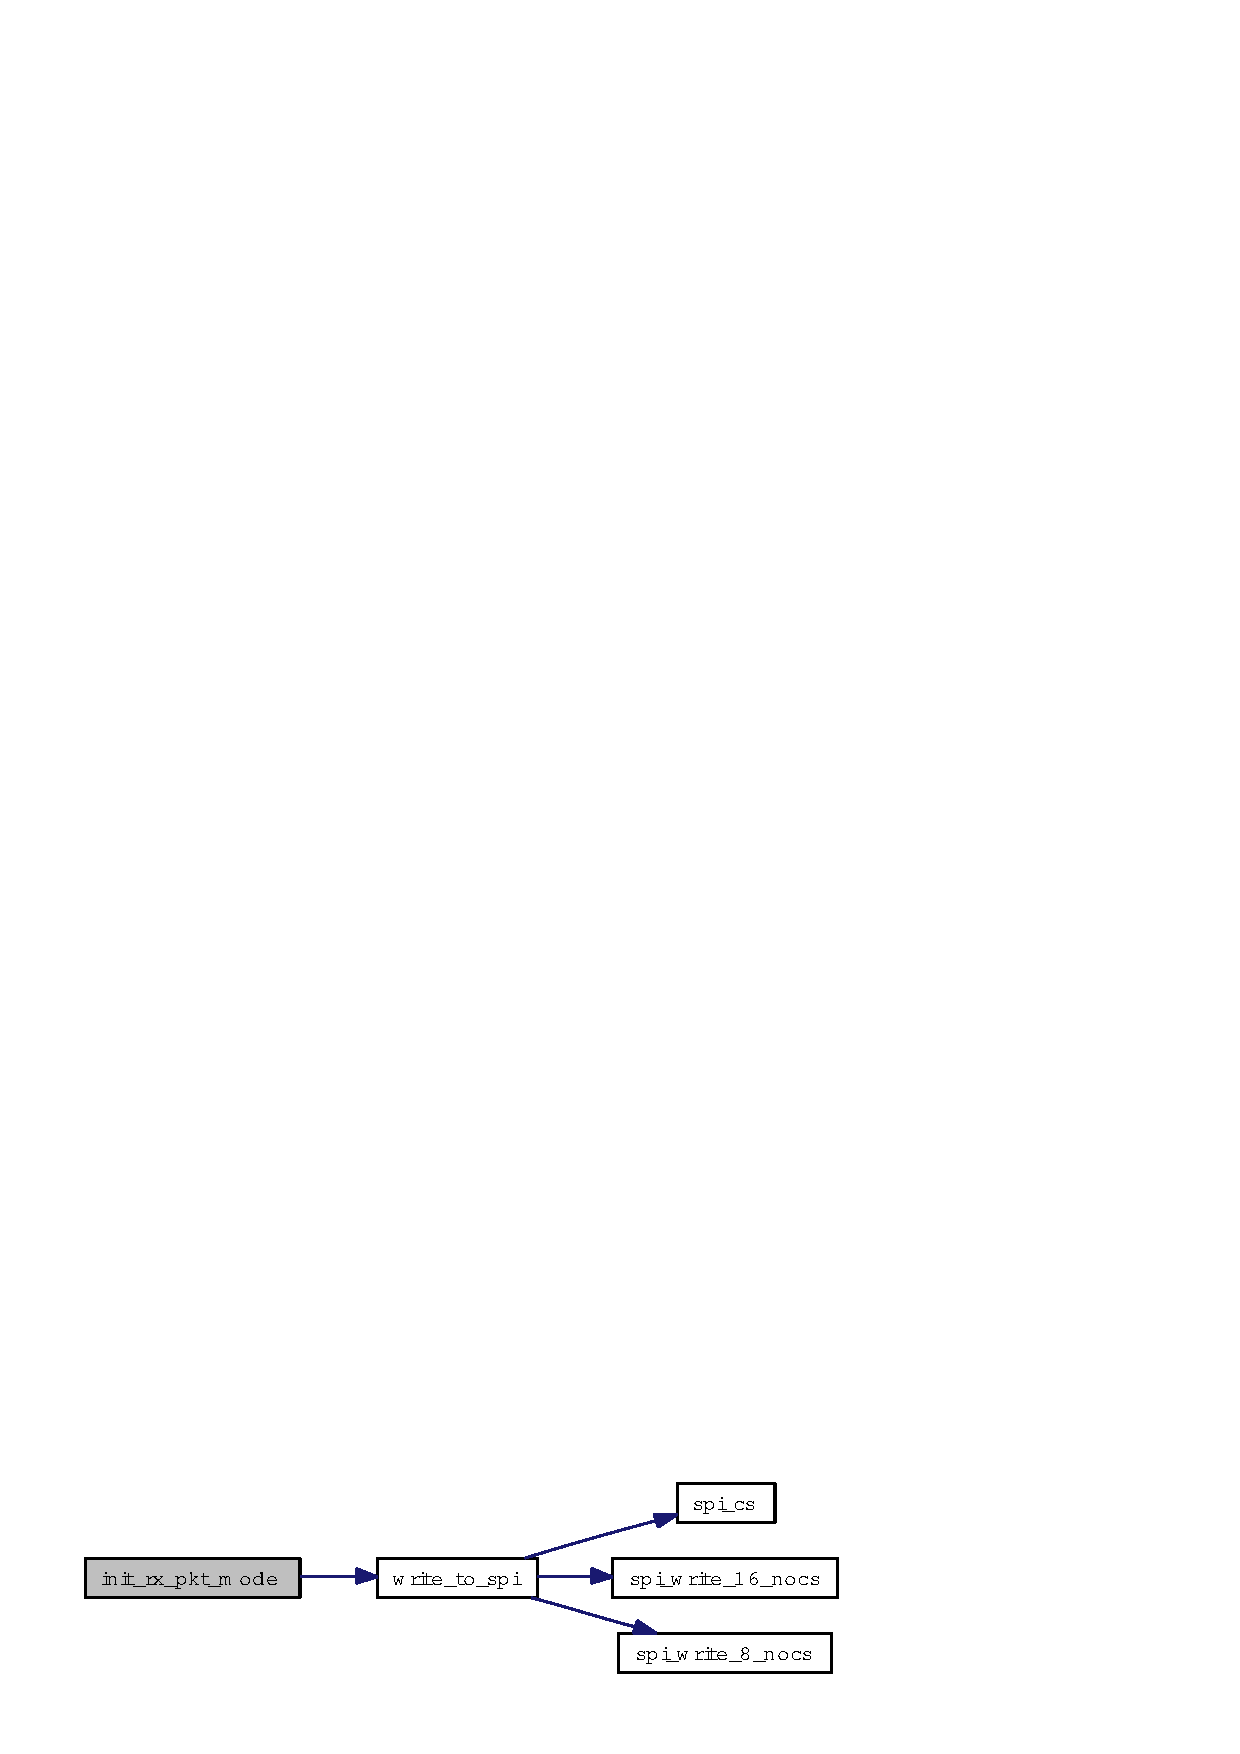
\includegraphics[width=203pt]{group__ro__transceiver__mac_g0ed60622e56ffb790ac27c0a3aa933ba_cgraph}
\end{center}
\end{figure}
\index{ro_transceiver_mac@{ro\_\-transceiver\_\-mac}!MC13192_init@{MC13192\_\-init}}
\index{MC13192_init@{MC13192\_\-init}!ro_transceiver_mac@{ro\_\-transceiver\_\-mac}}
\subsubsection{\setlength{\rightskip}{0pt plus 5cm}void MC13192\_\-init ()}\label{group__ro__transceiver__mac_g3b645fe6ce22a066678c3b54cfd59fef}


Initialize the MC13192 TODO: write detailed code description! 



Definition at line 36 of file transceiver\_\-mac.c.

References MC13192\_\-IDLE, mc13192\_\-mode, mc13192\_\-state, NO\_\-PACKET, read\_\-from\_\-spi(), and write\_\-to\_\-spi().

Referenced by main().

Here is the call graph for this function:\begin{figure}[H]
\begin{center}
\leavevmode
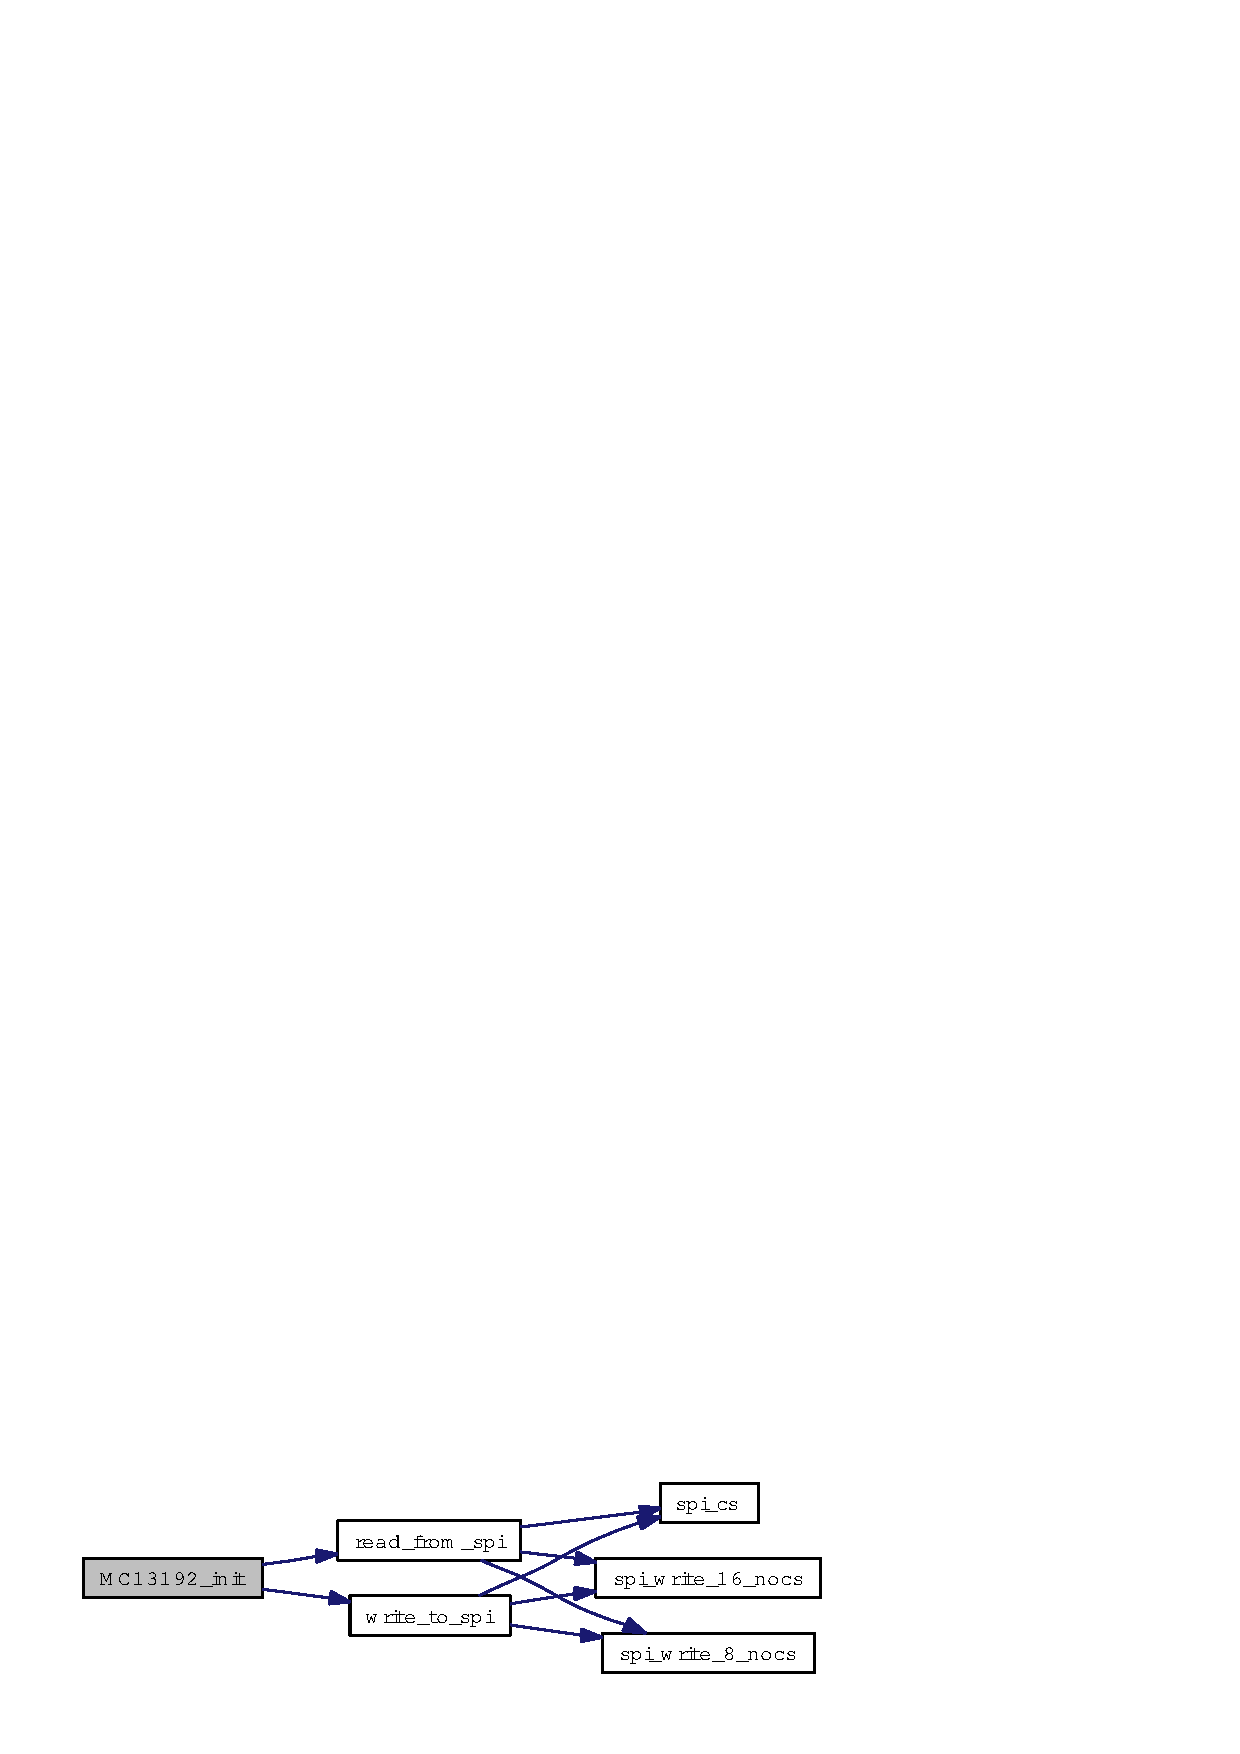
\includegraphics[width=199pt]{group__ro__transceiver__mac_g3b645fe6ce22a066678c3b54cfd59fef_cgraph}
\end{center}
\end{figure}
\index{ro_transceiver_mac@{ro\_\-transceiver\_\-mac}!MC13192_update_state@{MC13192\_\-update\_\-state}}
\index{MC13192_update_state@{MC13192\_\-update\_\-state}!ro_transceiver_mac@{ro\_\-transceiver\_\-mac}}
\subsubsection{\setlength{\rightskip}{0pt plus 5cm}void MC13192\_\-update\_\-state (void)}\label{group__ro__transceiver__mac_gafaa0125c377951f9b1599d1fb22f8a3}


Update the state variable to reflect the state of MC13192. 

$\ast$ TODO: write detailed code description! 

Definition at line 59 of file transceiver\_\-mac.c.

References DROP\_\-PACKET, mc13192\_\-state, NO\_\-PACKET, read\_\-from\_\-spi(), RX\_\-PACKET, and TX\_\-PACKET.

Here is the call graph for this function:\begin{figure}[H]
\begin{center}
\leavevmode
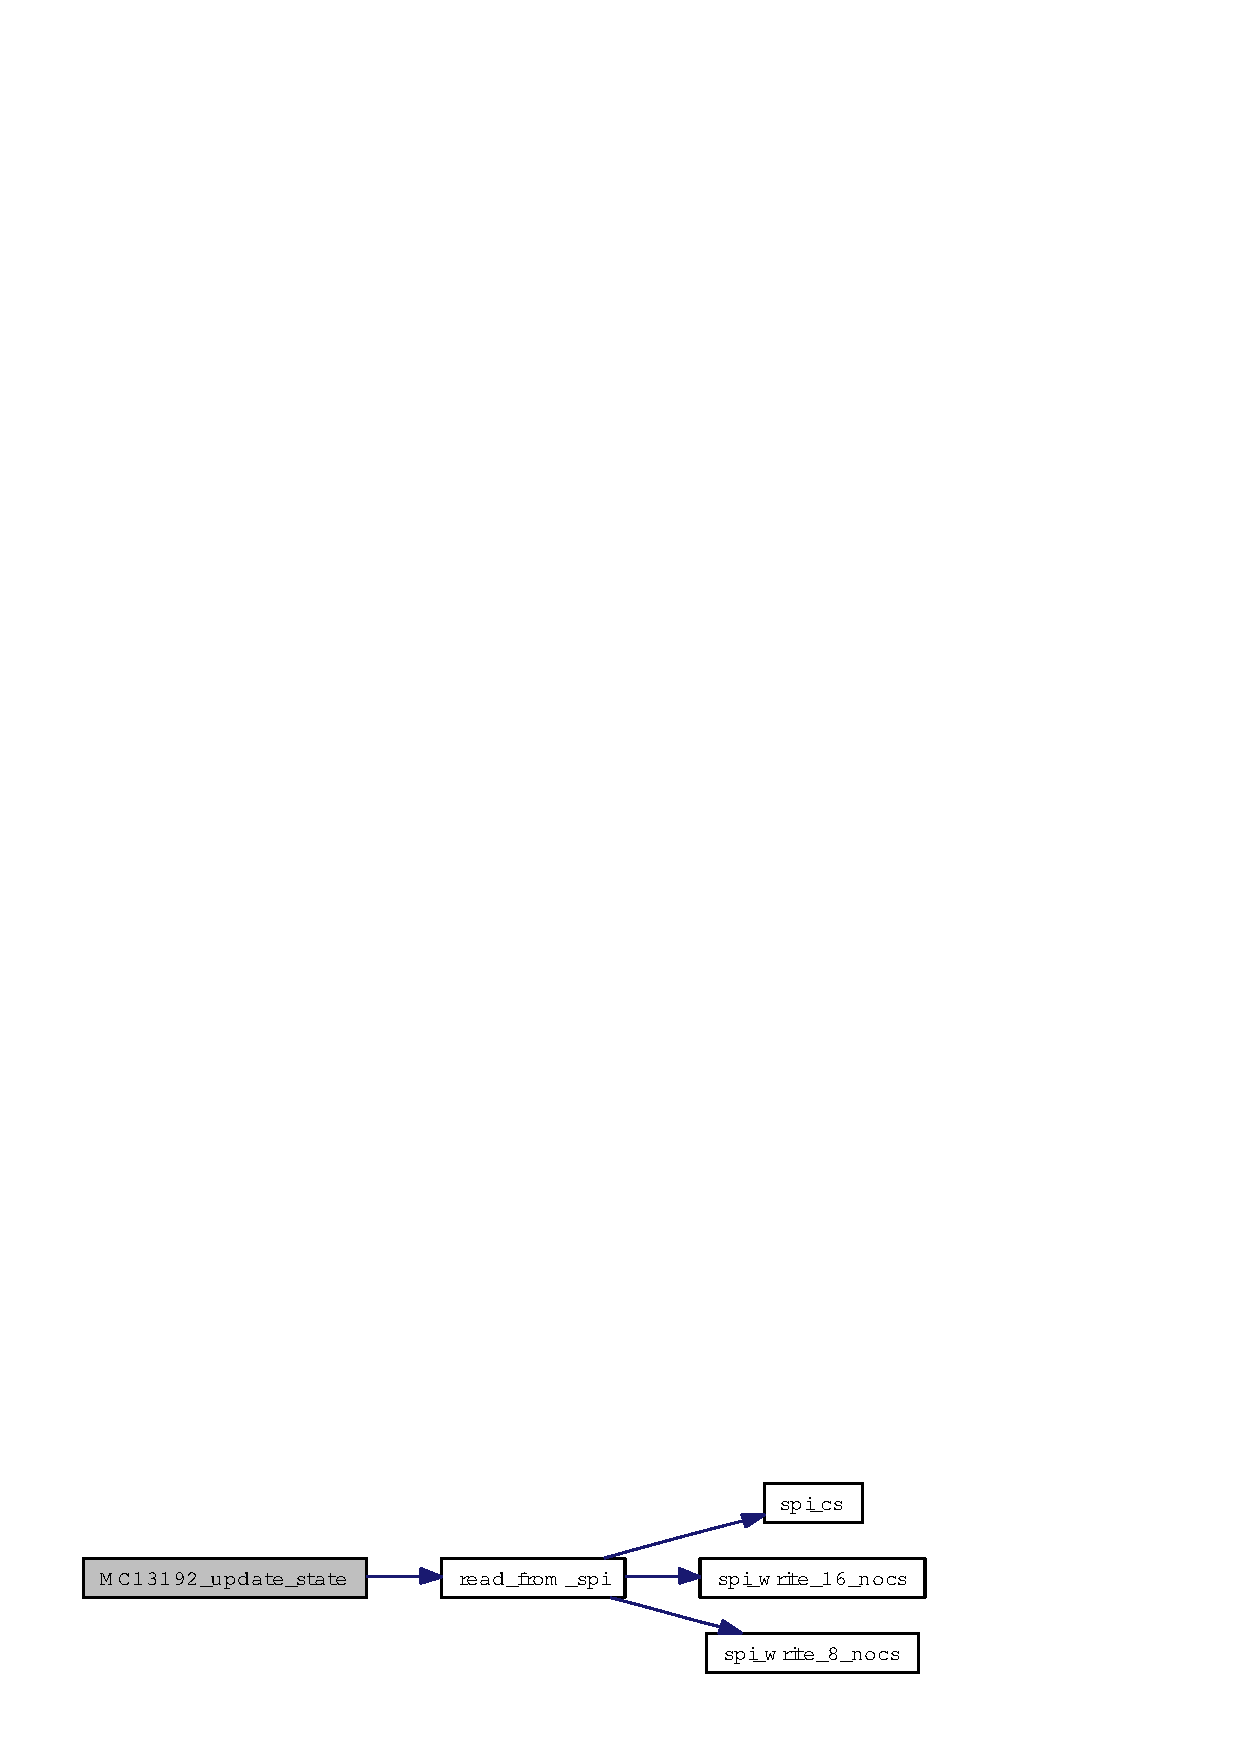
\includegraphics[width=224pt]{group__ro__transceiver__mac_gafaa0125c377951f9b1599d1fb22f8a3_cgraph}
\end{center}
\end{figure}
\index{ro_transceiver_mac@{ro\_\-transceiver\_\-mac}!tx_pkt_mode@{tx\_\-pkt\_\-mode}}
\index{tx_pkt_mode@{tx\_\-pkt\_\-mode}!ro_transceiver_mac@{ro\_\-transceiver\_\-mac}}
\subsubsection{\setlength{\rightskip}{0pt plus 5cm}int tx\_\-pkt\_\-mode ({\bf tx\_\-packet\_\-t} $\ast$ {\em tx\_\-packet})}\label{group__ro__transceiver__mac_g4a51cc343802a2c66a234e3d5b74f25c}


send a data packet TODO: write detailed code description! 

\begin{Desc}
\item[Parameters:]
\begin{description}
\item[{\em tx\_\-packet}]\end{description}
\end{Desc}


Definition at line 132 of file transceiver\_\-mac.c.

References tx\_\-packet\_\-t::data\-Length, write\_\-to\_\-ram(), and write\_\-to\_\-spi().

Here is the call graph for this function:\begin{figure}[H]
\begin{center}
\leavevmode
\includegraphics[width=194pt]{group__ro__transceiver__mac_g4a51cc343802a2c66a234e3d5b74f25c_cgraph}
\end{center}
\end{figure}


\subsection{Variable Documentation}
\index{ro_transceiver_mac@{ro\_\-transceiver\_\-mac}!mc13192_mode@{mc13192\_\-mode}}
\index{mc13192_mode@{mc13192\_\-mode}!ro_transceiver_mac@{ro\_\-transceiver\_\-mac}}
\subsubsection{\setlength{\rightskip}{0pt plus 5cm}uint8\_\-t {\bf mc13192\_\-mode}}\label{group__ro__transceiver__mac_gb358a2092e31591e6d721330d453c425}




Definition at line 33 of file transceiver\_\-mac.c.

Referenced by MC13192\_\-init().\index{ro_transceiver_mac@{ro\_\-transceiver\_\-mac}!mc13192_state@{mc13192\_\-state}}
\index{mc13192_state@{mc13192\_\-state}!ro_transceiver_mac@{ro\_\-transceiver\_\-mac}}
\subsubsection{\setlength{\rightskip}{0pt plus 5cm}uint8\_\-t {\bf mc13192\_\-state}}\label{group__ro__transceiver__mac_g553f7a0964d662b41a5fd9d9d782bdd2}




Definition at line 34 of file transceiver\_\-mac.c.

Referenced by MC13192\_\-init(), and MC13192\_\-update\_\-state().